% THIS DOCUMENT IS TAILORED TO REQUIREMENTS FOR SCIENTIFIC COMPUTING.  IT SHOULDN'T
% BE USED FOR NON-SCIENTIFIC COMPUTING PROJECTS
\documentclass[12pt]{article}

\usepackage{amsmath, mathtools}
\usepackage{amsfonts}
\usepackage{amssymb}
\usepackage{graphicx}
\usepackage{colortbl}
\usepackage{xr}
\usepackage{hyperref}
\usepackage{cleveref}
\usepackage{longtable}
\usepackage{xfrac}
\usepackage{tabularx}
\usepackage{ltablex}
\usepackage{float}
\usepackage{siunitx}
\usepackage{booktabs}
\usepackage{caption}
\usepackage{pdflscape}
\usepackage{afterpage}
\usepackage[version=4]{mhchem}
\usepackage{tikz}
\usetikzlibrary{positioning}

%\usepackage[round]{natbib}

%\usepackage{refcheck}

\crefformat{footnote}{#2\footnotemark[#1]#3}

\hypersetup{
    bookmarks=true,         % show bookmarks bar?
      colorlinks=true,       % false: boxed links; true: colored links
    linkcolor=red,          % color of internal links (change box color with linkbordercolor)
    citecolor=green,        % color of links to bibliography
    filecolor=magenta,      % color of file links
    urlcolor=cyan           % color of external links
}

%% Comments

\usepackage{color}

\newif\ifcomments\commentstrue %displays comments
%\newif\ifcomments\commentsfalse %so that comments do not display

\ifcomments
\newcommand{\authornote}[3]{\textcolor{#1}{[#3 ---#2]}}
\newcommand{\todo}[1]{\textcolor{red}{[TODO: #1]}}
\else
\newcommand{\authornote}[3]{}
\newcommand{\todo}[1]{}
\fi

\newcommand{\wss}[1]{\authornote{blue}{SS}{#1}} 
\newcommand{\plt}[1]{\authornote{magenta}{TPLT}{#1}} %For explanation of the template
\newcommand{\sjc}[1]{\authornote{cyan}{SC}{#1}}
%% Common Parts

\newcommand{\progname}{Master of Applied Science} 
\newcommand{\authname}{ChemCode
\\ Samuel Crawford}

\usepackage{hyperref}
    \hypersetup{colorlinks=true, linkcolor=blue, citecolor=blue, filecolor=blue,
                urlcolor=blue, unicode=false}
    \urlstyle{same}
                                

% For easy change of table widths
\newcommand{\colZwidth}{1.0\textwidth}
\newcommand{\colAwidth}{0.13\textwidth}
\newcommand{\colBwidth}{0.82\textwidth}
\newcommand{\colCwidth}{0.1\textwidth}
\newcommand{\colDwidth}{0.05\textwidth}
\newcommand{\colEwidth}{0.8\textwidth}
\newcommand{\colFwidth}{0.17\textwidth}
\newcommand{\colGwidth}{0.5\textwidth}
\newcommand{\colHwidth}{0.28\textwidth}

% Used so that cross-references have a meaningful prefix
\newcounter{defnum} %Definition Number
\newcommand{\dthedefnum}{GD\thedefnum}
\newcommand{\dref}[1]{GD\ref{#1}}
\newcounter{datadefnum} %Datadefinition Number
\newcommand{\ddthedatadefnum}{DD\thedatadefnum}
\newcommand{\ddref}[1]{DD\ref{#1}}
\newcounter{theorynum} %Theory Number
\newcommand{\tthetheorynum}{TM\thetheorynum}
\newcommand{\tref}[1]{TM\ref{#1}}
\newcounter{tablenum} %Table Number
\newcommand{\tbthetablenum}{TB\thetablenum}
\newcommand{\tbref}[1]{TB\ref{#1}}
\newcounter{assumpnum} %Assumption Number
\newcommand{\atheassumpnum}{P\theassumpnum}
\newcommand{\aref}[1]{A\ref{#1}}
\newcounter{goalnum} %Goal Number
\newcommand{\gthegoalnum}{P\thegoalnum}
\newcommand{\gsref}[1]{GS\ref{#1}}
\newcounter{instnum} %Instance Number
\newcommand{\itheinstnum}{IM\theinstnum}
\newcommand{\iref}[1]{IM\ref{#1}}
\newcounter{reqnum} %Requirement Number
\newcommand{\rthereqnum}{P\thereqnum}
\newcommand{\rref}[1]{R\ref{#1}}
\newcounter{nfrnum} %NFR Number
\newcommand{\rthenfrnum}{NFR\thenfrnum}
\newcommand{\nfrref}[1]{NFR\ref{#1}}
\newcounter{lcnum} %Likely change number
\newcommand{\lthelcnum}{LC\thelcnum}
\newcommand{\lcref}[1]{LC\ref{#1}}
\newcounter{ucnum} %Unlikely change number
\newcommand{\ltheucnum}{UC\theucnum}
\newcommand{\ucref}[1]{UC\ref{#1}}

\usepackage{fullpage}

\newcommand{\deftheory}[9][Not Applicable]
{
\noindent \rule{\textwidth}{0.5mm}
\paragraph{Number: } TM\refstepcounter{theorynum}\thetheorynum
\phantomsection \label{#2}

\paragraph{Label:} #3

\noindent \rule{\textwidth}{0.5mm}

\paragraph{Equation:}

#4

\paragraph{Description:}

#5

\paragraph{Notes:}

#6

\paragraph{Source:}

#7

\paragraph{Ref.\ By:}

#8

\paragraph{Derivation for \tref{#2}:}

#9

\noindent \rule{\textwidth}{0.5mm}

}

\begin{document}

\title{Software Requirements Specification for \progname:\\
  A program for solving chemistry problems}
\author{\authname}
\date{\today}

\maketitle
\thispagestyle{empty}

~\newpage

\pagenumbering{roman}

\tableofcontents

~\newpage

\section{Revision History} \label{sec_revHist}

\begin{tabularx}{\textwidth}{p{2.5cm}p{1.5cm}X}
  \toprule {\bf Date} & {\bf Version} & {\bf Notes}                                                          \\
  \midrule
  Jan. 21, 2023       & 0.0           & Start document, fill in title page, and add references               \\
                      & 0.1.0         & Fill in \nameref{sec_probDesc} and \nameref{sec_goals} sections, as
  well as all relevant definitions                                                                           \\
  Jan. 22, 2023       & 0.1.1         & Replace the notion of ``fractional oxidation state'' with
  ``nonstoichiometric compound''                                                                             \\
                      & 0.1.2         & Fix capTemplate reference                                            \\
                      & 0.2.0         & Update \nameref{srs_sec_abbsAcrs}                                    \\
                      & 0.2.1         & Add IM for balancing a chemical reaction (\iref{balance}), along
  with relevant reference information                                                                        \\
  Jan. 23, 2023       & 0.2.2         & Add IM for determining if a chemical reaction is feasible
  (\iref{feasible}), along with relevant reference information                                               \\
  Jan. 25, 2023       & 0.2.3         & Add references between sections for notation and
  definitions                                                                                                \\
                      & 0.2.4         & Abstract \iref{feasible}                                             \\
                      & 0.2.5         & Add IM for converting chemical equation to a matrix
  (\iref{convert}), along with relevant reference information                                                \\
                      & 0.2.6         & Rename and add input constraint to \iref{balance}                    \\
                      & 0.2.7         & Add note about \iref{balance} returning the smallest solution        \\
                      & 0.2.8         & Add TM for matrix equation (\tref{TM_MatEq})                         \\
                      & 0.2.9         & Improve referencing, mainly for TMs, and add note about
  potential TM for Conservation of Mass                                                                      \\
                      & 0.3.0         & Add check for Conservation of Mass in \iref{feasible}                \\
  Jan. 26, 2023       & 0.3.1         & Add \nameref{sec_LCs} from Problem Statement, add
  assumption about difference between number of elements and compounds
  (\aref{A_elemCompDiff}), and add mole to \nameref{sec_ToU}                                                 \\
                      & 0.3.2         & Update \tref{TM_MatEq} (and TM function) from feedback from
  presentation                                                                                               \\
                      & 0.3.3         & Fill in \nameref{sec_scope}, fix \aref{A_elemCompDiff} and
  change ``infeasible'' to ``feasible''                                                                      \\
  Jan. 27, 2023       & 0.4.0         & Improve section referencing in \nameref{sec_revHist}                 \\
                      & 0.4.1         & Fill in \nameref{sec_funcReqs}                                       \\
  Jan. 28, 2023       & 0.4.2         & Fill in main \nameref{sec_nonfuncReqs}, along with
  relevant reference information                                                                             \\
                      & 0.4.3         & Add TM for the Law of Conservation of Mass
  (\tref{TM_ConsMass})                                                                                       \\
                      & 0.4.4         & Represent input to \iref{convert} as two sequences of chemical
  formulas, add assumptions about user input, and remove infeasible
  likely change                                                                                              \\
  Jan. 29, 2023       & 0.5.0         & Add NFRs for understandability
  (\nfrref{NFR_understandability}) and verifiability
  (\nfrref{NFR_verifiability}) and improve quality of other NFRs                                             \\
  \bottomrule~                                                                                               \\
  ~                                                                                                          \\
  \toprule {\bf Date} & {\bf Version} & {\bf Notes}                                                          \\
  \midrule
  Jan. 29, 2023       & 0.5.1         & Fill in \nameref{sec_intro} based on Drasil examples                 \\
                      & 0.5.2         & Fill in \nameref{sec_phySystDesc} and remove ``product'' and
  ``reactant'' from \nameref{sec_termsDefs}                                                                  \\
  Jan. 30, 2023       & 0.5.3         & Remove unnecessary template comments about SRS document
  and the ones from \nameref{sec_specSysDesc} up to \nameref{sec_instance}                                   \\
                      & 0.5.4         & Remove unnecessary content from \nameref{sec_tabSymbs} and
  add the notion of ``gram'' to the document                                                                 \\
                      & 0.6.0         & Make \nfrref{NFR_accuracy} more accurate to current scope with
  potential future information for stretch goals added in comment                                            \\
                      & 0.6.1         & Make System Context diagram (Figure \ref{fig_sysCon}) and start
  to fill in \nameref{sec_sysCon}                                                                            \\
  Jan. 31, 2023       & 0.6.2         & Fill in rest of \nameref{sec_genSysDesc}                             \\
  Feb. 1, 2023        & 0.6.3         & Change abbreviation of theoretical model from ``T'' to
  ``TM'' and make TM references consistent with other references                                             \\
  Feb. 2, 2023        & 0.6.4         & Fill in \nameref{sec_refMat}, renaming specific matrices/vectors
  in \nameref{sec_instance}                                                                                  \\
                      & 0.6.5         & Reformat and clarify \nameref{sec_LCs}                               \\
  Feb. 3, 2023        & 0.6.6         & Add type notation and information                                    \\
                      & 0.6.7         & Fill in \nameref{sec_UCs}, add likely change for identifying
  more types of reactions (\lcref{LC_classMoreRxns}), and reference \aref{A_elemCompDiff} in \iref{convert}  \\
                      & 0.6.8         & Fill in \nameref{sec_traceMats} and remove more unnecessary content  \\
                      & 1.0           & Fill in data constraints sections, update traceability matrices, and
  finalize formatting                                                                                        \\
  Feb. 14, 2023       & 1.1.0         & Improve mathematical notation
  (remove ``$\times 1$'' from vector types, define $\mathbb{R}$) and citations                               \\
                      & 1.1.1         & Improve requirements based on feedback                               \\
  \bottomrule
\end{tabularx}

~\newpage

\section{Reference Material} \label{sec_refMat}

This section records information for easy reference.

\subsection{Table of Units} \label{sec_ToU}

Throughout this document, SI (Syst\`{e}me International d'Unit\'{e}s) is employed
as the unit system.
% In addition to the basic units, 
Several derived units are
used as described below.  For each unit, the symbol is given, followed by a
description of the unit and the SI name.
~\newline

\renewcommand{\arraystretch}{1.2}
%\begin{table}[ht]
\noindent \begin{tabular}{l l l}
  \toprule
  \textbf{symbol} & \textbf{unit}       & \textbf{SI} \\
  \midrule
  \si{\gram}      & mass                & gram        \\
  \si{\mole}      & amount of substance & mole        \\
  %    \si{\celsius} & temperature & centigrade\\
  %    \si{\watt} & power & watt (W = \si{\joule\per\second})\\
  \bottomrule
\end{tabular}
%	\caption{Provide a caption}
%\end{table}

% \plt{Derived units should show their derivation (the units they are derived
%   from) if their constituent units are used in the document. The symbol for units
%   named after people use capital letters, but the name
%   of the unit itself uses lower case. The one exception to this is degree Celsius.
%   Details on writing metric units can be found on the
%   \href{https://www.nist.gov/pml/weights-and-measures/writing-metric-units}
%   {NIST} web-page.}

\subsection{Table of Symbols} \label{sec_tabSymbs}

The table that follows summarizes the symbols used in this document along with
their units and types. The choice of symbols was made to be consistent with
linear algebra conventions while distinguishing between specific matrices.  The
symbols are listed in alphabetical order.

% \renewcommand{\arraystretch}{1.2}
\noindent \begin{tabularx}{\textwidth}{l l l X} \toprule
  \textbf{symbol} & \textbf{unit} & \textbf{type}             & \textbf{description}                             \\
  \midrule
  $\textbf{0}$    & --            & $\mathbb{N}^{m}$          & zero vector                                      \\
  $\textbf{A}$    & --            & $\mathbb{R}^{m \times n}$ & generic matrix                                   \\
  $\textbf{E}$    & --            & $\mathbb{R}^{m \times n}$ & matrix representation of a chemical equation     \\
  $\textbf{b}$    & --            & $\mathbb{R}^{m}$          & generic vector                                   \\
  $\textbf{c}$    & --            & $(\mathbb{Z^+})^{n}$      & vector of the smallest coefficients that balance
  a chemical equation                                                                                            \\
  $m$             & --            & $\mathbb{Z}^+$            & generic whole number                             \\
  $n$             & --            & $\mathbb{Z}^+$            & generic whole number                             \\
  $\textbf{x}$    & --            & $\mathbb{R}^{n}$          & generic vector                                   \\
  \bottomrule
\end{tabularx}

\subsection{Abbreviations and Acronyms} \label{srs_sec_abbsAcrs}

\renewcommand{\arraystretch}{1.2}
\begin{tabular}{l l}
  \toprule
  \textbf{symbol} & \textbf{description}                \\
  \midrule
  % 1D              & One-Dimensional                     \\
  A               & Assumption                          \\
  DD              & Data Definition                     \\
  GD              & General Definition                  \\
  GS              & Goal Statement                      \\
  IM              & Instance Model                      \\
  LC              & Likely Change                       \\
  PS              & Physical System Description         \\
  R               & Requirement                         \\
  SRS             & Software Requirements Specification \\
  TM              & Theoretical Model                   \\
  VnV             & Verification and Validation         \\
  \bottomrule
\end{tabular}\\

\subsection{Mathematical Notation} \label{sec_mathNot}

Matrices are written in bold uppercase letters (for example $\textbf{A}$), while
vectors (one-dimensional matrices) are written in bold lowercase letters, (for
example
$\textbf{x}$) \cite{osullivan_appendix_2010}. The type of a matrix will be
denoted by the type of each value in the matrix with the matrix's dimensions
as a superscript; for example, a matrix of natural numbers with two rows and
three columns is of type $\mathbb{N}^{2 \times 3}$
\cite[p.~3]{golub_matrix_2013}. Since vectors are one-dimensional
matrices, their types only have one dimension; for example, a row vector with
four entries is denoted by $\mathbb{N}^{4}$ \cite[p.~4]{golub_matrix_2013}.
The zero matrix is a special
type of matrix where each element is zero and is denoted by $\textbf{0}$
\cite{weisstein_zero_2023}.
% Individual entries in a matrix are written in
% lowercase letters with their row and column number, in that order, written as
% subscripts (for example $a_{12}$) \cite{osullivan_appendix_2010}; these
% subscripts are sometimes separated by a comma for clarity (for example
% $a_{12,34}$) \cite{latecki_matrices_2018}. 
Two (or more) matrices with the same
number of rows can be joined together to form an ``augmented matrix'', written
as $\left(\textbf{A}\vert \textbf{B}\right)$ \cite{taboga_augmented_2021}.

The set of natural numbers is denoted by $\mathbb{N}$ and consists of the
non-negative integers (including zero). The set of whole numbers is denoted by
$\mathbb{Z}^+$ and consists of the positive integers (excluding zero). The
set of real numbers is denoted by $\mathbb{R}$ and consists of every number
``that can be expressed as an infinite decimal expansion''
\cite{the_editors_of_encyclopaedia_britannica_real_2022}.

% \plt{If symbols are used to show mathematical operations,
%   these should be summarized here.  In some cases the easiest way to summarize
%   the notation is to point to a text or other source that explains the
%   notation.}

\newpage

\pagenumbering{arabic}

%\plt{An SRS document should have the following qualities: unambiguous,
%  consistent, complete, validatable, abstract and traceable. Intended readers
%	 (Section~\ref{sec_IntendedReader}) should be able to learn,
%  understand and verify the captured domain knowledge, as well as 
%  independently verify/derive every statement made.}

\section{Introduction} \label{sec_intro}
Chemical equations are common ways of representing chemical reactions (as
described in \nameref{sec_phySystDesc}), but must be balanced for use in other
calculations \cite{lund_introduction_2023}. Therefore, it is useful to have a
tool to automatically balance these chemical reactions for efficiency and
accuracy.

The following section provides an overview of the Software Requirements
Specification (SRS) for \progname{}. This section explains the purpose of this
document, the scope of the requirements, the characteristics of the intended
reader, and the organization of the document.

\subsection{Purpose of Document}

The primary purpose of this document is to record the requirements of the
program for solving chemistry problems \sjc{Is this a good description?}.
Goals, assumptions, theoretical models,
definitions, and other model derivation information are specified, allowing the
reader to fully understand and verify the purpose and scientific basis of
\progname{}. With the exception of system constraints, this SRS will remain
abstract, describing what problem is being solved, but not how to solve it.

This document will be used as a starting point for subsequent development
phases, including writing the design specification and the software Verification
and Validation (VnV) Plan. The design document will show how the requirements
are to be realized, including decisions on the numerical algorithms and
programming environment. The VnV Plan will show the steps that will be used to
increase confidence in the software documentation and the implementation.
Although the SRS fits in a series of documents that follow the so-called
``waterfall model'', the actual development process is not constrained in any
way. Even when the waterfall model is not followed, as Parnas and Clements point
out in \cite{ParnasAndClements1986}, the most logical way to present the
documentation is still to ``fake'' a rational design process.

\subsection{Scope of Requirements} \label{sec_scope}

The scope of the requirements includes determining if a given chemical equation
is feasible (see \nameref{sec_termsDefs}) and, if it is, balancing it using the
smallest whole number coefficients possible, regardless of whether or not the
chemical formulas in the equation are correct or if the reaction would take
place in a real-world setting.

\subsection{Characteristics of Intended Reader} \label{sec_IntendedReader}
Reviewers of this documentation should have an understanding of high-school level
chemistry, namely stoichiometry (see \nameref{sec_termsDefs}), and undergraduate
Level 1 linear algebra, namely solving systems of linear equations. The end user
of \progname{}, as described in \nameref{sec_userChars}, does not require
knowledge of linear algebra, since relevant concepts will be implemented by the
code and hidden from the user.

\subsection{Organization of Document}
The organization of this document is based on a template from
\cite{smith_captemplate_2022}, which is based on the template for an SRS for
scientific computing software proposed by \cite{SmithAndLai2005},
\cite{SmithEtAl2007}, and \cite{koothoor_document_2013}. The presentation
follows the standard pattern of presenting goals, theories, definitions, and
assumptions. For readers that would like a more bottom-up approach, they can
start reading the \nameref{sec_instance} and trace back to find any additional
information they require.

The \nameref{sec_goals} are refined to the \nameref{sec_theoretical}, which are
refined to the \nameref{sec_instance}.

\section{General System Description} \label{sec_genSysDesc}

This section provides general information about the system.  It identifies the
interfaces between the system and its environment, describes the user
characteristics and lists the system constraints.

\subsection{System Context} \label{sec_sysCon}
\begin{figure}[h!]
  \begin{center}
    \begin{tikzpicture}[
        roundnode/.style={circle, draw=black, very thick, minimum size=20mm},
        squarednode/.style={rectangle, draw=black, very thick, minimum size=20mm},
      ]
      %Nodes
      \node[roundnode]        (user_input)                              {User};
      \node[squarednode, xshift = 3cm]      (\progname{})       [right=of user_input] {\progname{}};
      \node[roundnode, xshift = 3cm]        (user_output)       [right=of \progname{}] {User};
      \node[roundnode, align=center, yshift = 1.5cm] (ext_lib) [above=of \progname{}] {External\\Library};
      \node[roundnode, draw=none, align=center, yshift = 1.538cm] (upArrow) [above=of \progname{}] {};\node[roundnode, draw=none, align=center, yshift = 1.55cm] (downArrow) [above=of \progname{}] {};

      %Lines
      \draw[->, very thick] (user_input.east) -- (\progname{}.west) node[above, pos=0.5, align=center] {An unbalanced\\chemical equation};
      \begin{scope}[transform canvas={xshift=-.7em}]
        \draw[->, very thick] (\progname{}.north) -- (upArrow.south) node[left, pos=0.5, align=right] {The chemical\\equation as\\ a matrix};
      \end{scope}
      \begin{scope}[transform canvas={xshift=.7em}]
        \draw[->, very thick] (downArrow.south) -- (\progname{}.north) node[right, pos=0.5, align=left] {The matrix\\ after processing\\};
      \end{scope}
      \draw[->, very thick] (\progname{}.east) -- (user_output.west) node[above, pos=0.5, align=center] {A balanced\\form of the\\chemical equation};
    \end{tikzpicture}
    \caption{System Context}
    \label{fig_sysCon}
  \end{center}
\end{figure}

Figure \ref{fig_sysCon} shows the system context. A circle represents an
external entity outside the software. A rectangle represents the software system
itself (\progname{}). Arrows are used to show the data flow between the system
and its environment.

\begin{itemize}
  \item User Responsibilities:
        \begin{itemize}
          \item Provide an unbalanced chemical equation, ensuring conformation to input
                data format required by \progname{}
          \item Ensure required software assumptions from Subsection~\ref{sec_assumps}
                are appropriate for the problem to which the user is applying the software
        \end{itemize}
  \item \progname{} Responsibilities:
        \begin{itemize}
          \item Detect data type mismatch, such as a string of characters instead of a
                rational number
          \item Detect improperly formatted chemical equations
          \item Format inputted chemical equation as a matrix
          \item Determine if the inputted chemical equation is feasible
          \item If the inputted chemical equation is feasible, find its balanced form with
                the smallest whole number coefficients
        \end{itemize}
  \item External Library Responsibilities:
        \begin{itemize}
          \item Process the chemical equation matrix \sjc{Can this be more descriptive?}
        \end{itemize}
\end{itemize}

\subsection{User Characteristics} \label{sec_userChars}

The end user of \progname{} should have an understanding of high-school level
chemistry, namely stoichiometry (see \nameref{sec_termsDefs}).

\subsection{System Constraints} \label{sec_sysConst}

%\plt{System constraints differ from other type of requirements because they
%  limit the developers' options in the system design and they identify how the
%  eventual system must fit into the world. This is the only place in the SRS
%  where design decisions can be specified.  That is, the quality requirement for
%  abstraction is relaxed here.  However, system constraints should only be
%  included if they are truly required.}

\progname~will be developed using Drasil \cite{carette_drasil_2021}, ``a
framework for generating high-quality documentation and code for Scientific
Computing Software'' \cite[p. iii]{maclachlan_design_2020}, with the goal of
extending it by adding concepts relevant to the problem outlined in
\nameref{sec_probDesc}. One of the desired additions to Drasil is the notion of
systems of linear equations, so this problem will be solved using matrices.
Since Drasil is built on the idea of reusability, external libraries will be
used to solve these systems of linear equations. This was previously done with
ordinary differential equation (ODE) solvers, since ``creating a complete ODE
solver in Drasil would take considerable time, and there are already many
reliable external libraries \dots tested by long use''
\cite[p. 24]{chen_solving_2022}; these rationales also apply to solvers of
systems of linear equations.

\section{Specific System Description} \label{sec_specSysDesc}

This section first presents the problem description, which gives a high-level
view of the problem to be solved.  This is followed by the solution characteristics
specification, which presents the assumptions, theories, definitions and finally
the instance models.

\subsection{Problem Description} \label{sec_probDesc}

\progname{} is intended to balance chemical equations (including ones with
nonstoichiometric compounds; see \nameref{sec_termsDefs}) so
they can be useful for other computations \cite{lund_introduction_2023}.
Additionally, since molecules only exist in whole numbers (since dividing a
molecule changes its composition into new types of molecules), the coefficients
used to balance the equation must be whole
numbers, and by convention should be as small as possible
\cite{lund_introduction_2023}.

\subsubsection{Terminology and  Definitions} \label{sec_termsDefs}
This subsection provides a list of terms that are used in the subsequent
sections and their meaning, with the purpose of reducing ambiguity and making it
easier to correctly understand the requirements:

\begin{itemize}
  \item \textbf{Feasible}: (Referring to a chemical equation) able to be
        balanced \cite{hamid_balancing_2019}.

  \item \textbf{Hydrate}: ``A compound formed by the chemical combination of water
        and some other substance in a definite molecular ratio''
        \cite{harpercollins_publishers_hydrate_nodate}.

  \item \textbf{Nonstoichiometric Compound}: ``Any solid chemical compound in
        which the numbers of atoms of the elements present cannot be expressed as a
        ratio of small whole numbers''
        \cite{the_editors_of_encyclopaedia_britannica_nonstoichiometric_2010}.

  \item \textbf{Stoichiometry}: ``The calculation of the quantities of reactants
        or products in a chemical reaction using the relationships found in a balanced
        chemical equation'' \cite[p. 337]{lund_introduction_2023}.

        %\item \textbf{Reduced Row Echelon Form}: A form of a matrix where every row
        %with only zeros is at the bottom and every column but the rightmost one
        %has all zeroes except for one one (which has only zeroes to its left)
        %\cite{taboga_reduced_2021}.
\end{itemize}

\subsubsection{Physical System Description} \label{sec_phySystDesc}

Chemical reactions are interactions between different types of matter that
result in new substances being formed \cite[p. 286]{lund_introduction_2023}.
These are represented using chemical equations, with the reactant(s)---the
substance(s) present at the beginning of the reaction---on the left-hand side
and the product(s)---the substance(s) formed by the reaction---on the right. An
example of a chemical equation representing the combustion of methane in the
presence of oxygen to form carbon dioxide and water vapour is shown below. The
subscripts indicate how many of each element is present in the given chemical
compound.
$$
  \ce{CH4} + \ce{O2} \rightarrow \ce{CO2} + \ce{H2O}
$$

\sjc{Is this paragraph helpful/needed?} As mentioned in
\nameref{sec_probDesc}, chemical formulas must be balanced to be
useful in other reactions \cite{lund_introduction_2023}. This means that there
must be the same number of each element before and after the reaction takes
place to satisfy the Law of Conservation of Mass (\tref{TM_ConsMass}). Since
changing the subscripts in a formula will change the type of molecule (for
example, \ce{O3} is ozone, not oxygen), equations are balanced by introducing
coefficients before each compound. If no coefficient is present, there is an
implicit coefficient of ``1''. The above equation looks like this in its
balanced form:
$$
  \ce{CH4} + \ce{2O2} \rightarrow \ce{CO2} + \ce{2H2O}
$$

The physical system of \progname{} includes:

\begin{itemize}

  \item[PS1:] the products of a given chemical reaction;

  \item[PS2:] the reactants of the same chemical reaction.

\end{itemize}

% \begin{figure}[h!]
% \begin{center}
% %\rotatebox{-90}
% {
%  \includegraphics[width=0.5\textwidth]{<FigureName>}
% }
% \caption{\label{<Label>} <Caption>}
% \end{center}
% \end{figure}

\subsubsection{Goal Statements} \label{sec_goals}
Given a representation of a chemical equation, the goal statements
of \progname{} are:

\begin{itemize}

  \item[GS\refstepcounter{goalnum}\thegoalnum \label{G_feasible}:] Determine if
    a given chemical reaction is feasible (see \nameref{sec_termsDefs}).

  \item[GS\refstepcounter{goalnum}\thegoalnum \label{G_balance}:] Balance the
    inputted chemical equation with the smallest whole number coefficients
    possible.

\end{itemize}

\subsection{Solution Characteristics Specification}

%\plt{DDs are not refined; they are just used. DDs are not derived; they are
%	just given. If a potential DD includes a derivation, then that means it is
%	refining other models, which would make it a GD or an IM. TMs are also just
%	given, but they are refined, not used.}
%
%\noindent \plt{The relationships between the parts of the document are show in
%  the following figure.  In this diagram ``may ref'' has the same role as
%  ``uses'' above.  The figure adds ``Likely Changes,'' which are able to
%  reference (use) Assumptions.}
%
%\begin{figure}[H]
%  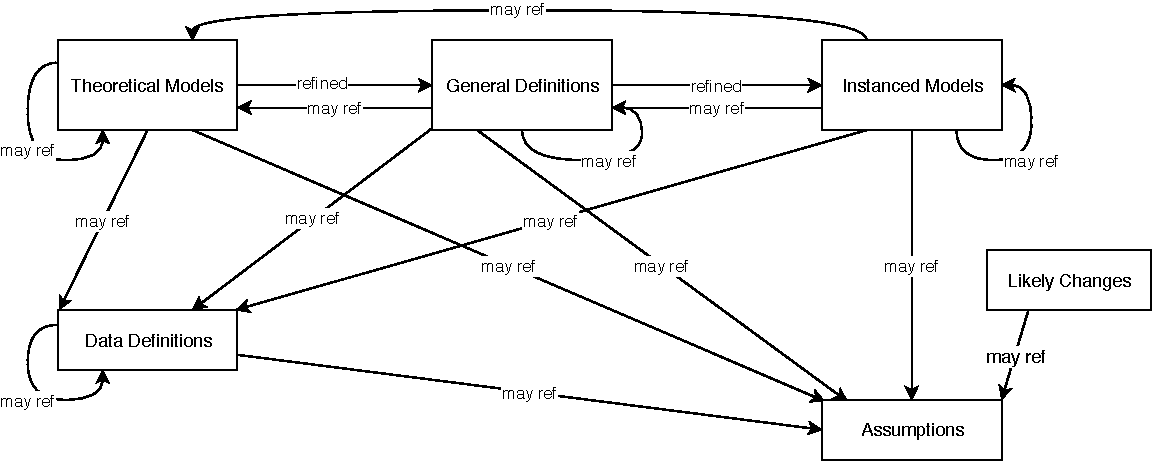
\includegraphics[scale=0.9]{RelationsBetweenTM_GD_IM_DD_A.pdf}
%\end{figure}

The instance models that govern \progname{} are presented in
Subsection~\ref{sec_instance}.  The information to understand the meaning of the
instance models and their derivation is also presented, so that the instance
models can be verified.

\subsubsection{Assumptions} \label{sec_assumps}

This section simplifies the original problem and helps in developing the
theoretical model by filling in the missing information for the physical
system. The numbers given in the square brackets refer to the theoretical model
  [TM], general definition [GD], data definition [DD], instance model [IM],
likely change [LC], or unlikely change [UC] in which the respective assumption
is used.

\begin{itemize}

  \item[A\refstepcounter{assumpnum}\theassumpnum \label{A_elemCompDiff}:]
    For all inputted chemical equations, there is at most one more compound than
    element. \sjc{Should this be an assumption or a requirement?}
    [\iref{convert}, \ucref{UC_allEqsPermitted}]

  \item[A\refstepcounter{assumpnum}\theassumpnum \label{A_validInput}:]
    All inputted chemical formulas describe real chemical formulas.
      [\iref{convert}]

  \item[A\refstepcounter{assumpnum}\theassumpnum \label{A_correctInputFormat}:]
    All inputted chemical formulas are formatted following some set of
    agreed-upon conventions.	[\iref{convert}, \lcref{LC_incorrectInputFormat}]

  \item[A\refstepcounter{assumpnum}\theassumpnum \label{A_simpleForms}:]
    All inputted chemical formulas are simple; i.e., only consist of atomic symbols
    and subscripts.	[\iref{convert}, \lcref{LC_complexForms}]

\end{itemize}

\newpage

\subsubsection{Theoretical Models}\label{sec_theoretical}

%\plt{Theoretical models are sets of abstract mathematical equations or axioms
%  for solving the problem described in \nameref{sec_phySystDesc}. Examples of
%  theoretical models are
%  physical laws, constitutive equations, relevant conversion factors, etc.}

This section focuses on the general equations and laws that \progname{} is based
on.

\noindent
\deftheory
% #2 refname of theory
{TM_MatEq}
% #3 label
{Matrix equation}
% #4 equation
{
  $\textbf{A}\textbf{x}=\textbf{b}$
}
% #5 description
{
  The above equation gives the general form of the matrix equation where
  $\textbf{A}$ is of type $\mathbb{R}^{m\times n}$, $\textbf{b}$ is of type
  $\mathbb{R}^{m}$, and $\textbf{x}$ is of type
  $\mathbb{R}^{n}$. \sjc{Is this type information redundant to have
    here?} The values of $\textbf{x}$ are unknown
  and will be solved for \cite{margalit_matrix_2019}.
}
% #6 Notes
{
  For any $\textbf{A}$ and $\textbf{b}$, there is either zero, one, or infinite
  values for $\textbf{x}$ \cite{zwick_math_2012}.
}
% #7 Source
{
  \url{https://textbooks.math.gatech.edu/ila/matrix-equations.html}
}
% #8 Referenced by
{
  \iref{balance}
}
% #9 derivation - not applicable by default
{Not Applicable}

\newpage
\noindent
\deftheory
% #2 refname of theory
{TM_ConsMass}
% #3 label
{Law of Conservation of Mass}
% #4 equation
{Not Applicable}
% #5 description
{
  This law states that ``matter can neither be created nor destroyed in a
  chemical reaction \dots but it may change forms to other substances''
  \cite[p. 112]{lund_introduction_2023}.
}
% #6 Notes
{None}
% #7 Source
{
  \url{https://chem.libretexts.org/Courses/Anoka-Ramsey_Community_College/Introduction_to_Chemistry/03\%3A_Matter_and_Energy/3.06\%3A_Conservation_of_Mass}
}
% #8 Referenced by
{
  \iref{feasible}
}
% #9 derivation - not applicable by default
{Not Applicable}

%\noindent
%\deftheory
%% #2 refname of theory
%{TM_COE}
%% #3 label
%{Conservation of thermal energy}
%% #4 equation
%{
%  $-{\bf \nabla \cdot q} + g$ = $\rho C \frac{\partial T}{\partial t}$
%}
%% #5 description
%{
%  The above equation gives the conservation of energy for transient heat transfer in a material
%  of specific heat capacity $C$ (\si{\joule\per\kilogram\per\celsius}) and density $\rho$ 
%  (\si{\kilogram\per\cubic\metre}), where $\bf q$ is the thermal flux vector (\si{\watt\per\square\metre}),
%  $g$ is the volumetric heat generation
%  (\si{\watt\per\cubic\metre}), $T$ is the temperature
%  (\si{\celsius}),  $t$ is time (\si{\second}), and $\nabla$ is
%  the gradient operator.  For this equation to apply, other forms
%  of energy, such as mechanical energy, are assumed to be negligible in the
%  system (\aref{A_OnlyThermalEnergy}).  In general, the material properties ($\rho$ and $C$) depend on temperature.
%}
%% #6 Notes
%{
%None.
%}
%% #7 Source
%{
%  \url{http://www.efunda.com/formulae/heat_transfer/conduction/overview_cond.cfm}
%}
%% #8 Referenced by
%{
%  \dref{ROCT}
%}
%% #9 derivation - not applicable by default
%{Not Applicable}

\subsubsection{General Definitions}\label{sec_gendef}

%\plt{Generally the reduction
%  in abstraction is possible through invoking (using/referencing) Assumptions.
%  For instance, the TM could be Newton's Law of Cooling stated abstracting.  The
%  GD could take the general law and apply it to get a 1D equation.}

%This section collects the laws and equations that will be used in building the
%instance models.

There are no general definitions.

%\noindent
%\begin{minipage}{\textwidth}
%\renewcommand*{\arraystretch}{1.5}
%\begin{tabular}{| p{\colAwidth} | p{\colBwidth}|}
%\hline
%\rowcolor[gray]{0.9}
%Number& GD\refstepcounter{defnum}\thedefnum \label{NL}\\
%\hline
%Label &\bf Newton's law of cooling \\
%\hline
%% Units&$MLt^{-3}T^0$\\
%% \hline
%SI Units&\si{\watt\per\square\metre}\\
%\hline
%Equation&$ q(t) = h \Delta T(t)$  \\
%\hline
%Description &
%Newton's law of cooling describes convective cooling from a surface.  The law is
%stated as: the rate of heat loss from a body is proportional to the difference
%in temperatures between the body and its surroundings.
%\\
%& $q(t)$ is the thermal flux (\si{\watt\per\square\metre}).\\
%& $h$ is the heat transfer coefficient, assumed independent of $T$ (\aref{A_hcoeff})
%	(\si{\watt\per\square\metre\per\celsius}).\\
%&$\Delta T(t)$= $T(t) - T_{\text{env}}(t)$ is the time-dependent thermal gradient
%between the environment and the object (\si{\celsius}).
%\\
%\hline
%  Source & Citation here \\
%  \hline
%  Ref.\ By & \ddref{FluxCoil}, \ddref{FluxPCM}\\
%  \hline
%\end{tabular}
%\end{minipage}\\
%
%\subsubsection*{Detailed derivation of simplified rate of change of temperature}
%
%\plt{This may be necessary when the necessary information does not fit in the
%  description field.}
%\plt{Derivations are important for justifying a given GD.  You want it to be
%  clear where the equation came from.}

\subsubsection{Data Definitions}\label{sec_datadef}

%\plt{The Data Definitions are definitions of symbols and equations that are
%  given for the problem.  They are not derived; they are simply used by other
%  models.}
%
%This section collects and defines all the data needed to build the instance
%models. The dimension of each quantity is also given.

There are no data definitions.

%\noindent
%\begin{minipage}{\textwidth}
%\renewcommand*{\arraystretch}{1.5}
%\begin{tabular}{| p{\colAwidth} | p{\colBwidth}|}
%\hline
%\rowcolor[gray]{0.9}
%Number& DD\refstepcounter{datadefnum}\thedatadefnum \label{FluxCoil}\\
%\hline
%Label& \bf Heat flux out of coil\\
%\hline
%Symbol &$q_C$\\
%\hline
%% Units& $Mt^{-3}$\\
%% \hline
%  SI Units & \si{\watt\per\square\metre}\\
%  \hline
%  Equation&$q_C(t) = h_C (T_C - T_W(t))$, over area $A_C$\\
%  \hline
%  Description & 
%                $T_C$ is the temperature of the coil (\si{\celsius}).  $T_W$ is the temperature of the water (\si{\celsius}).  
%                The heat flux out of the coil, $q_C$ (\si{\watt\per\square\metre}), is found by
%                assuming that Newton's Law 
%                of Cooling applies (\aref{A_Newt_coil}).  This law (\dref{NL}) is used on the surface of
%                the coil, which has area $A_C$ (\si{\square\metre}) and heat 
%                transfer coefficient $h_C$
%                (\si{\watt\per\square\metre\per\celsius}).  This equation
%                assumes that the temperature of the coil is constant over time (\aref{A_tcoil}) and that it does not vary along the length
%                of the coil (\aref{A_tlcoil}).
%  \\
%  \hline
%  Sources& Citation here \\
%  \hline
%  Ref.\ By & \iref{ewat}\\
%  \hline
%\end{tabular}
%\end{minipage}\\

% \subsubsection{Data Types}\label{sec_datatypes}

% \plt{This section is optional.  In many scientific computing programs it isn't
%   necessary, since the inputs and outputs are straightforward types, like reals,
%   integers, and sequences of reals and integers.  However, for some problems it
%   is very helpful to capture the type information.}

% \plt{The data types are not derived; they are simply stated and used by other
%   models.}

% \plt{All data types must be used by at least one of the models.}

% \plt{For the mathematical notation for expressing types, the recommendation is
%   to use the notation of~\cite{HoffmanAndStrooper1995}.}

% This section collects and defines all the data types needed to document the
% models. \plt{Modify the examples below for your problem, and add additional
%   definitions as appropriate.}

% ~\newline

% \noindent
% \begin{minipage}{\textwidth}
%   \renewcommand*{\arraystretch}{1.5}
%   \begin{tabular}{| p{\colAwidth} | p{\colBwidth}|}
%     \hline
%     \rowcolor[gray]{0.9}
%     Type Name   & Name for Type                                              \\
%     \hline
%     Type Def    & mathematical definition of the type                        \\
%     \hline
%     Description & description here
%     \\
%     \hline
%     Sources     & Citation here, if the type is borrowed from another source \\
%     \hline
%   \end{tabular}
% \end{minipage}\\

\subsubsection{Instance Models} \label{sec_instance}

This section transforms the problem defined in \nameref{sec_probDesc} into
one which is expressed in mathematical terms. It uses concrete symbols defined
in Section~\ref{sec_datadef} to replace the abstract symbols in the models
identified in Sections~\ref{sec_theoretical} and~\ref{sec_gendef} \sjc{Should
  the reference to the general models be removed if there aren't any?}.

The goals \gsref{G_feasible} and \gsref{G_balance} are solved by \iref{feasible}
and \iref{balance}, respectively.

~\newline

%\noindent
%\begin{minipage}{\textwidth}
%\renewcommand*{\arraystretch}{1.5}
%\begin{tabular}{| p{\colAwidth} | p{\colBwidth}|}
%  \hline
%  \rowcolor[gray]{0.9}
%  Number& IM\refstepcounter{instnum}\theinstnum \label{ewat}\\
%  \hline
%  Label& \bf Energy balance on water to find $T_W$\\
%  \hline
%  Input&$m_W$, $C_W$, $h_C$, $A_C$, $h_P$, $A_P$, $t_\text{final}$, $T_C$, 
%  $T_\text{init}$, $T_P(t)$ from \iref{epcm}\\
%  & The input is constrained so that $T_\text{init} \leq T_C$ (\aref{A_charge})\\
%  \hline
%  Output&$T_W(t)$, $0\leq t \leq t_\text{final}$, such that\\
%  &$\frac{dT_W}{dt} = \frac{1}{\tau_W}[(T_C - T_W(t)) + {\eta}(T_P(t) - T_W(t))]$,\\
%  &$T_W(0) = T_P(0) = T_\text{init}$ (\aref{A_InitTemp}) and $T_P(t)$ from \iref{epcm} \\
%  \hline
%  Description&$T_W$ is the water temperature (\si{\celsius}).\\
%  &$T_P$ is the PCM temperature (\si{\celsius}).\\
%  &$T_C$ is the coil temperature (\si{\celsius}).\\
%  &$\tau_W = \frac{m_W C_W}{h_C A_C}$ is a constant (\si{\second}).\\
%  &$\eta = \frac{h_P A_P}{h_C A_C}$ is a constant (dimensionless).\\
%  & The above equation applies as long as the water is in liquid form,
%  $0<T_W<100^o\text{C}$, where $0^o\text{C}$ and $100^o\text{C}$ are the melting
%  and boiling points of water, respectively (\aref{A_OpRange}, \aref{A_Pressure}).
%  \\
%  \hline
%  Sources& Citation here \\
%  \hline
%  Ref.\ By & \iref{epcm}\\
%  \hline
%\end{tabular}
%\end{minipage}\\
%
%%~\newline
%
%\subsubsection*{Derivation of ...}
%
%\plt{The derivation shows how the IM is derived from the TMs/GDs.  In cases
%  where the derivation cannot be described under the Description field, it will
%  be necessary to include this subsection.}

\noindent
\begin{minipage}{\textwidth}
  \renewcommand*{\arraystretch}{1.5}
  \begin{tabular}{| p{\colAwidth} | p{\colBwidth}|}
    \hline
    \rowcolor[gray]{0.9}
    Number      & IM\refstepcounter{instnum}\theinstnum \label{convert}              \\
    \hline
    Label       & \bf Matrix representation of elements present in reaction          \\
    \hline
    Input       & Two sequences of representations of chemical formulas; one for the
    reactants and one for the products.                                              \\
    \hline
    Output      & \textbf{E}, a matrix such that each entry
    indicates the amount of a given element in a given compound; each row
    corresponds to a different element and each column corresponds to a different
    compound. Positive entries indicate the compound is a reactant, negative
    entries indicate the compound is a product, and zeroes indicate the
    corresponding element is not present in the corresponding compound.              \\
    \hline
    Description & Each chemical formula present in the inputted sequences are
    assumed to be valid (\aref{A_validInput}), be formatted correctly
    (\aref{A_correctInputFormat}), and only consist of atomic symbols and
    subscripts (\aref{A_simpleForms}). The number of columns is assumed to be
    at most one more than the number of rows (\aref{A_elemCompDiff}).
    \\
    \hline
    Sources     & \cite{hamid_balancing_2019}                                        \\
    \hline
    Ref.\ By    & \iref{feasible}, \iref{balance}                                    \\
    \hline
  \end{tabular}
\end{minipage}\\

~\newline

%\subsubsection*{Derivation of ...}
%
%\plt{The derivation shows how the IM is derived from the TMs/GDs.  In cases
%  where the derivation cannot be described under the Description field, it will
%  be necessary to include this subsection.}

\noindent
\begin{minipage}{\textwidth}
  \renewcommand*{\arraystretch}{1.5}
  \begin{tabular}{| p{\colAwidth} | p{\colBwidth}|}
    \hline
    \rowcolor[gray]{0.9}
    Number      & IM\refstepcounter{instnum}\theinstnum \label{feasible}               \\
    \hline
    Label       & \bf Determination of feasibility                                     \\
    \hline
    Input       & $\textbf{E}$ from \iref{convert}                                     \\
    %  & The input is constrained so that $T_\text{init} \leq T_C$ (\aref{A_charge})\\
    \hline
    Output      & $\textsc{F}$ if a row of $\textbf{E}$ does not have a positive and a
    negative entry or if $(\textbf{E} \vert \textbf{0})$ has no solutions and
    $\textsc{T}$ otherwise                                                             \\
    \hline
    Description & $\textbf{E}$ is a matrix representing the amount of each element
    in each compound in a reaction from \iref{convert}. \sjc{Is this necessary?}
    If a row of $\textbf{E}$ only has either a positive or negative entry, then
    there is an element that is either a reactant or a product but not both,
    which breaks the Law of Conservation of
    Mass (\tref{TM_ConsMass}). \sjc{Is this a good place for this?}                    \\
    %  &$\textbf{R}$ is the $m \times n$ matrix $(\textbf{A} \vert \textbf{0})$
    %  as close to reduced row echelon form (see \nameref{sec_termsDefs}) as possible
    %  from \iref{epcm}.
    %	\sjc{Is the relationship between $\textbf{R}$ and $r_{m,n-1}$ clear?}
    %  \sjc{Where should $\textbf{R}$ be defined?}\\
                & $\textbf{0}$ is the zero matrix (see \nameref{sec_mathNot}).         \\
    %  & The above equation applies as long as the water is in liquid form,
    %  $0<T_W<100^o\text{C}$, where $0^o\text{C}$ and $100^o\text{C}$ are the melting
    %  and boiling points of water, respectively (\aref{A_OpRange}, \aref{A_Pressure}).
    %  \\
    \hline
    Sources     & \cite{hamid_balancing_2019}                                          \\
    %  , \cite{pramoditha_how_2021} \\
    \hline
    Ref.\ By    & \iref{balance}, \ucref{UC_diffSolveMethod}                           \\
    \hline
  \end{tabular}
\end{minipage}\\

~\newline
%
%\subsubsection*{Derivation of ...}
%
%\plt{The derivation shows how the IM is derived from the TMs/GDs.  In cases
%  where the derivation cannot be described under the Description field, it will
%  be necessary to include this subsection.}

\noindent
\begin{minipage}{\textwidth}
  \renewcommand*{\arraystretch}{1.5}
  \begin{tabular}{| p{\colAwidth} | p{\colBwidth}|}
    \hline
    \rowcolor[gray]{0.9}
    Number      & IM\refstepcounter{instnum}\theinstnum \label{balance}                \\
    \hline
    Label       & \bf Vector of compound coefficients in balanced equation             \\
    \hline
    Input       & $\textbf{E}$ from \iref{convert}                                     \\
                & The input is constrained so that $\textbf{E}$ is feasible
    (\iref{feasible}).
    \sjc{Is this correct?}                                                             \\
    \hline
    Output      & $\textbf{c}$, such that it is the smallest solution to               \\
                & $\textbf{E}\textbf{c} = \textbf{0}$ from \tref{TM_MatEq}
    %  \sjc{TM refs not working.}
    \sjc{Is this sufficient?}                                                          \\
    \hline
    Description & $\textbf{E}$ is a matrix representing the amount of each element
    in each compound in a reaction from \iref{convert}. \sjc{Is this necessary?}       \\
                & $\textbf{c}$ is a vector of whole number coefficients for each
    compound in the reaction (in the order inputted) so that the equation is balanced. \\
                & $\textbf{0}$ is the zero matrix (see \nameref{sec_mathNot}).         \\
    %  & The above equation applies as long as the water is in liquid form,
    %  $0<T_W<100^o\text{C}$, where $0^o\text{C}$ and $100^o\text{C}$ are the melting
    %  and boiling points of water, respectively (\aref{A_OpRange}, \aref{A_Pressure}).
    %  \\
    \hline
    Sources     & \cite{hamid_balancing_2019}                                          \\
    \hline
    Ref.\ By    & \ucref{UC_diffSolveMethod}                                           \\
    \hline
  \end{tabular}
\end{minipage}\\

%~\newline

%\subsubsection*{Derivation of ...}
%
%\plt{The derivation shows how the IM is derived from the TMs/GDs.  In cases
%  where the derivation cannot be described under the Description field, it will
%  be necessary to include this subsection.}

\subsubsection{Input Data Constraints} \label{sec_DataConst}

There are no input data constraints.

% Table~\ref{TblInputVar} shows the data constraints on the input output
% variables.  The column for physical constraints gives the physical limitations
% on the range of values that can be taken by the variable.  The column for
% software constraints restricts the range of inputs to reasonable values.  The
% software constraints will be helpful in the design stage for picking suitable
% algorithms.  The constraints are conservative, to give the user of the model the
% flexibility to experiment with unusual situations.  The column of typical values
% is intended to provide a feel for a common scenario.  The uncertainty column
% provides an estimate of the confidence with which the physical quantities can be
% measured.  This information would be part of the input if one were performing an
% uncertainty quantification exercise.

% The specification parameters in Table~\ref{TblInputVar} are listed in
% Table~\ref{TblSpecParams}.

% \begin{table}[!h]
%   \caption{Input Variables} \label{TblInputVar}
%   \renewcommand{\arraystretch}{1.2}
%   \noindent \begin{longtable*}{l l l l c}
%     \toprule
%     \textbf{Var} & \textbf{Physical Constraints} & \textbf{Software Constraints} &
%     \textbf{Typical Value} & \textbf{Uncertainty}\\
%     \midrule
%     $L$ & $L > 0$ & $L_{\text{min}} \leq L \leq L_{\text{max}}$ & 1.5 \si[per-mode=symbol] {\metre} & 10\%
%     \\
%     \bottomrule
%   \end{longtable*}
% \end{table}

% \noindent
% \begin{description}
%   \item[(*)] \plt{you might need to add some notes or clarifications}
% \end{description}

% \begin{table}[!h]
%   \caption{Specification Parameter Values} \label{TblSpecParams}
%   \renewcommand{\arraystretch}{1.2}
%   \noindent \begin{longtable*}{l l}
%     \toprule
%     \textbf{Var} & \textbf{Value} \\
%     \midrule
%     $L_\text{min}$ & 0.1 \si{\metre}\\
%     \bottomrule
%   \end{longtable*}
% \end{table}

\subsubsection{Properties of a Correct Solution} \label{sec_PropsCorrSol}

The equation from \iref{balance} can be used as a ``sanity'' check, using the
original input (formatted as a matrix according to \iref{convert}) as
$\textbf{E}$ and the outputted vector of coefficients as $\textbf{c}$.
Performing this matrix multiplication should result in the zero matrix,
$\textbf{0}$.

% A correct solution must exhibit \plt{fill in the details}.  \plt{These
%   properties are in addition to the stated requirements.  There is no need to
%   repeat the requirements here.  These additional properties may not exist for
%   every problem.  Examples include conservation laws (like conservation of
%   energy or mass) and known constraints on outputs, which are usually summarized
%   in tabular form.  A sample table is shown in Table~\ref{TblOutputVar}}

% \begin{table}[!h]
%   \caption{Output Variables} \label{TblOutputVar}
%   \renewcommand{\arraystretch}{1.2}
%   \noindent \begin{longtable*}{l l}
%     \toprule
%     \textbf{Var} & \textbf{Physical Constraints} \\
%     \midrule
%     $T_W$ & $T_\text{init} \leq T_W \leq T_C$ (by~\aref{A_charge})
%     \\
%     \bottomrule
%   \end{longtable*}
% \end{table}

% \plt{This section is not for test cases or techniques for verification and
%   validation.  Those topics will be addressed in the Verification and Validation
%   plan.}

\newpage

\section{Requirements}
This section provides the functional requirements, the business tasks that the
software is expected to complete, and the nonfunctional requirements, the
qualities that the software is expected to exhibit.

\subsection{Functional Requirements} \label{sec_funcReqs}

\begin{itemize}

  \item[R\refstepcounter{reqnum}\thereqnum \label{R_input}:] Input a
    representation of a chemical equation.

  \item[R\refstepcounter{reqnum}\thereqnum \label{R_convert}:] Convert the
    inputted equation to matrix form (from \iref{convert}).

  \item[R\refstepcounter{reqnum}\thereqnum \label{R_feasible}:] Determine if the
    inputted equation is feasible (see \nameref{sec_termsDefs};	from
    \iref{feasible}).

  \item[R\refstepcounter{reqnum}\thereqnum \label{R_infeasOutput}:] If the
    inputted equation is infeasible, output a descriptive message.

  \item[R\refstepcounter{reqnum}\thereqnum \label{R_balance}:] If the
    inputted equation is feasible, balance the chemical equation with the smallest
    whole number coefficients possible (from \iref{balance}).

  \item[R\refstepcounter{reqnum}\thereqnum \label{R_feasOutput}:] If the
    inputted equation is feasible, output a balanced form of the equation in the
    same format as the input, using the coefficients from \iref{balance}.

    %\item[R\refstepcounter{reqnum}\thereqnum \label{R_VerifyOutput}:]
    %  \plt{Verification related requirements.}
\end{itemize}

%\plt{Every IM should map to at least one requirement, but not every requirement
%  has to map to a corresponding IM.}

\subsection{Nonfunctional Requirements} \label{sec_nonfuncReqs}

\begin{itemize}

  \item[NFR\refstepcounter{nfrnum}\thenfrnum \label{NFR_accuracy}:]
    \textbf{Accuracy:} Chemical equations are only useful if they are balanced
    \cite{lund_introduction_2023}, so computed coefficients from \iref{balance}
    should be exact.

    %  All other computed solutions should have a relative error no greater
    %  than 0.1\%, since the most finely-calibrated chemistry equipment has a
    %  relative error of 0.1-0.2\% \cite{walker_volumetric_2012,
    %  godambe_measuring_nodate}. Additionally, any fractional value calculated
    %  should be reported to the appropriate number of significant figures
    %  \cite{lund_introduction_2023}. \sjc{Specify what that means}

    %  \plt{Characterize the accuracy by giving the context/use for
    %    the software.  Maybe something like, ``The accuracy of the computed
    %    solutions should meet the level needed for $<$engineering or scientific
    %    application$>$.  The level of accuracy achieved by \progname{} shall be
    %    described following the procedure given in Section~X of the Verification and
    %    Validation Plan.''  A link to the VnV plan would be a nice extra.}

  \item[NFR\refstepcounter{nfrnum}\thenfrnum \label{NFR_understandability}:]
    \textbf{Understandability:} A new intended user (as described by
    \nameref{sec_userChars}) should be able to learn how to use \progname{} in an
    acceptable amount of time, as measured by the procedure in Section X of
    the Verification and Validation (VnV) Plan.

  \item[NFR\refstepcounter{nfrnum}\thenfrnum \label{NFR_usability}:]
    \textbf{Usability:} An intended user (as described by \nameref{sec_userChars})
    should find \progname{} easy to use, as measured by the procedure in Section X
    of the VnV Plan.

  \item[NFR\refstepcounter{nfrnum}\thenfrnum \label{NFR_maintainability}:]
    \textbf{Maintainability:} The development time for any of the likely
    changes should not exceed $\text{MAINTAIN\_FRAC}$ of the original
    development time.

  \item[NFR\refstepcounter{nfrnum}\thenfrnum \label{NFR_portability}:]
    \textbf{Portability:} \progname{} should be able to run on systems with the
    corresponding programming language
    installed, including systems running on Windows or macOS. The tests from
    the VnV Plan should pass in these environments.

  \item[NFR\refstepcounter{nfrnum}\thenfrnum \label{NFR_verifiability}:]
    \textbf{Verifiability:} \progname{} is tested following the VnV Plan.

    %\item Reusability?.

\end{itemize}

\newpage

\section{Likely Changes} \label{sec_LCs}

\begin{itemize}

  \item[LC\refstepcounter{lcnum}\thelcnum\label{LC_complexForms}:] The system
    currently assumes that inputted chemical formulas are simple
    (\aref{A_simpleForms}). In the future, the user might
    be able to input more complex chemical formulas, such as hydrates (see
    \nameref{sec_termsDefs}) or those with polymers or isotopes.

  \item[LC\refstepcounter{lcnum}\thelcnum\label{LC_calcMoles}:] In the future,
    \progname{} might be able to, given the amount of one substance (in moles)
    in a reaction, calculate the amount required/produced of every other
    substance (also in moles) in the reaction.\footnote{
      \label{chemProbExs}These examples of problems related to
      chemical equations were taken from \cite{lund_introduction_2023}.}

  \item[LC\refstepcounter{lcnum}\thelcnum\label{LC_detLimReag}:] In the future,
    \progname{} might be able to, given the amount
    of each reactant (in moles) in a reaction,
    determine the limiting reactant(s).\cref{chemProbExs}
    This is dependent on \lcref{LC_calcMoles}.

  \item[LC\refstepcounter{lcnum}\thelcnum\label{LC_calcYield}:] In the future,
    \progname{} might be able to, given the amount
    of more than one reactant (in moles) in a reaction,
    calculate the theoretical yield of each product (also in
    moles).\cref{chemProbExs} This is dependent on \lcref{LC_detLimReag}.

  \item[LC\refstepcounter{lcnum}\thelcnum\label{LC_calcExcess}:] In the future,
    \progname{} might be able to, given the amount
    of more than one reactant (in moles) in a reaction,
    calculate the amount of excess reactant(s) (also in	moles).\cref{chemProbExs}
    This is dependent on \lcref{LC_detLimReag}.

  \item[LC\refstepcounter{lcnum}\thelcnum\label{LC_incorrectInputFormat}:]
    The system currently assumes that inputted chemical formulas are formatted
    according to some set of conventions
    (\aref{A_correctInputFormat}). In the future, \progname{} might be able to
    parse valid but incorrectly formatted chemical formulas inputted by the
    user and format them correctly when outputting them.

  \item[LC\refstepcounter{lcnum}\thelcnum\label{LC_termsOfMass}:] In the future,
    the user might be able to enter the amounts required by \lcref{LC_calcMoles},
    \lcref{LC_detLimReag}, \lcref{LC_calcYield}, and \lcref{LC_calcExcess} in
    terms of mass (e.g., in grams).\cref{chemProbExs}

  \item[LC\refstepcounter{lcnum}\thelcnum\label{LC_classRxns}:] In the future,
    \progname{} might be able to classify a chemical reaction as ``combination
    (or synthesis), decomposition, combustion, single replacement, [or] double
    replacement'' \cite[p.~301]{lund_introduction_2023}.\cref{chemProbExs}

  \item[LC\refstepcounter{lcnum}\thelcnum\label{LC_classMoreRxns}:] In the
    future, \progname{} might also be able to classify ``oxidation-reduction
    reactions, \dots acid-base reactions, and condensation reactions''
    \cite[p.~301]{lund_introduction_2023}.\cref{chemProbExs} This should be
    done after \lcref{LC_classRxns}.

  \item[LC\refstepcounter{lcnum}\thelcnum\label{LC_inputPhaseLabels}:] In the
    future, \progname{} might allow the user to input phase
    labels.\cref{chemProbExs}

  \item[LC\refstepcounter{lcnum}\thelcnum\label{LC_identifyPhaseLabels}:] In
    the future, \progname{} might be able to, given the phase labels for the
    reactants of a reaction, identify the phase labels for the products, which
    would involve determining solubility.\cref{chemProbExs} This is dependent
    on \lcref{LC_inputPhaseLabels}.

  \item[LC\refstepcounter{lcnum}\thelcnum\label{LC_rxnTakePlace}:] In the
    future, \progname{} might be able to identify when a reaction will not take
    place.\cref{chemProbExs}
    This is dependent on \lcref{LC_identifyPhaseLabels}.

\end{itemize}

\section{Unlikely Changes} \label{sec_UCs}

\begin{itemize}

  \item[UC\refstepcounter{ucnum}\theucnum\label{UC_diffSolveMethod}:] One of
    the system constraints in Subsection~\ref{sec_sysConst} is that \progname{}
    will be implemented using matrices and linear algebra. It is unlikely that
    a different method will be used to compute the values from \iref{feasible}
    and \iref{balance}, since ``balancing chemical equations is not chemistry;
    it is just linear algebra'' \cite[p. 193]{risteski_new_2021}.

  \item[UC\refstepcounter{ucnum}\theucnum\label{UC_allEqsPermitted}:]
    \aref{A_elemCompDiff} assumes that for all inputted chemical equations,
    there is at most one more compound than element. Using WebQC's chemical
    equation balancer \cite{noauthor_balance_2023}, equations without this
    constraint, such as $\ce{O3} + \ce{C} \rightarrow \ce{O2} + \ce{CO2}$,
    ``can be balanced in an infinite number of ways'' and are
    ``combination[s] of two different reactions'' \cite{noauthor_balance_2023}.
    Manual empirical analysis of these equations led to unexpected results.
    The constraint in \aref{A_elemCompDiff} might be a law of nature and a
    byproduct of ``balancing chemical equations [being] just linear algebra''
    \cite[p. 193]{risteski_new_2021}, but preliminary investigation did not
    find any proof of this. Therefore, this constraint will remain an
    assumption and is unlikely to be relaxed.

\end{itemize}

\section{Traceability Matrices} \label{sec_traceMats}

The purpose of the traceability matrices is to provide easy references on what
has to be additionally modified if a certain component is changed.  Every time a
component is changed, the items in the column of that component that are marked
with an ``X'' may have to be modified as well. Table~\ref{Table:srs_trace} shows
the dependencies of theoretical models, general definitions, data definitions,
instance models, and data constraints on each other. Table~\ref{Table:A_trace}
shows the dependencies of theoretical models,
general definitions, data definitions, instance models, likely changes, and
unlikely changes on the assumptions. Table~\ref{Table:R_trace}
shows the dependencies of requirements on instance models.

\begin{table}[h!]
  \centering
  \begin{tabular}{|c|c|c|c|c|c|c|c|}
    \hline
                       & \tref{TM_MatEq} & \tref{TM_ConsMass} & \iref{convert} & \iref{feasible} & \iref{balance} & \ref{sec_DataConst} & \ref{sec_PropsCorrSol} \\
    \hline
    \tref{TM_MatEq}    &                 &                    &                &                 &                &                     &                        \\ \hline
    \tref{TM_ConsMass} &                 &                    &                &                 &                &                     &                        \\ \hline
    \iref{convert}     &                 &                    &                &                 &                &                     & X                      \\ \hline
    \iref{feasible}    &                 & X                  & X              &                 &                &                     &                        \\ \hline
    \iref{balance}     & X               &                    & X              & X               &                &                     & X                      \\ \hline
  \end{tabular}
  \caption{Traceability Matrix Showing the Connections Between Items of Different Sections}
  \label{Table:srs_trace}
\end{table}

\begin{table}[h!]
  \parbox{.45\linewidth}{
    \centering
    \begin{tabular}{|c|c|c|c|}%c|c|c|c|c|c|c|c|c|c|c|c|}
      \hline
                                     & \iref{convert} & \iref{feasible} & \iref{balance} \\ % & \rref{R_input} & \rref{R_convert} & \rref{R_feasible} & \rref{R_balance} & \rref{R_infeasOutput} & \rref{R_feasOutput} & \nfrref{NFR_accuracy} & \nfrref{NFR_understandability} & \nfrref{NFR_usability} & \nfrref{NFR_maintainability} & \nfrref{NFR_portability} & \nfrref{NFR_verifiability} \\
      \hline
      % \iref{convert}                 &&&&&&&&&&&&&&&&\\ \hline
      % \iref{feasible}                &X&&&&&&&&&&&&&&&\\ \hline
      % \iref{balance}                 &X&X&&&&&&&&&&&&&&\\ \hline
      \rref{R_input}                 &                &                 &                \\ \hline % &                &                  &                   &                  &                       &                     &                       &                                &                        &                              &                          &                            \\ \hline
      \rref{R_convert}               & X              &                 &                \\ \hline % &                &                  &                   &                  &                       &                     &                       &                                &                        &                              &                          &                            \\ \hline
      \rref{R_feasible}              &                & X               &                \\ \hline % &                &                  &                   &                  &                       &                     &                       &                                &                        &                              &                          &                            \\ \hline
      \rref{R_infeasOutput}          &                &                 &                \\ \hline % &                &                  &                   &                  &                       &                     &                       &                                &                        &                              &                          &                            \\ \hline
      \rref{R_balance}               &                &                 & X              \\ \hline % &                &                  &                   &                  &                       &                     &                       &                                &                        &                              &                          &                            \\ \hline
      \rref{R_feasOutput}            &                &                 & X              \\ \hline % &                &                  &                   &                  &                       &                     &                       &                                &                        &                              &                          &                            \\ \hline
      \nfrref{NFR_accuracy}          &                &                 & X              \\ \hline % &                &                  &                   &                  &                       &                     &                       &                                &                        &                              &                          &                            \\ \hline
      \nfrref{NFR_understandability} &                &                 &                \\ \hline % &                &                  &                   &                  &                       &                     &                       &                                &                        &                              &                          &                            \\ \hline
      \nfrref{NFR_usability}         &                &                 &                \\ \hline % &                &                  &                   &                  &                       &                     &                       &                                &                        &                              &                          &                            \\ \hline
      \nfrref{NFR_maintainability}   &                &                 &                \\ \hline % &                &                  &                   &                  &                       &                     &                       &                                &                        &                              &                          &                            \\ \hline
      \nfrref{NFR_portability}       &                &                 &                \\ \hline % &                &                  &                   &                  &                       &                     &                       &                                &                        &                              &                          &                            \\ \hline
      \nfrref{NFR_verifiability}     &                &                 &                \\ \hline % &                &                  &                   &                  &                       &                     &                       &                                &                        &                              &                          &                            \\ \hline
    \end{tabular}
    \caption{Traceability Matrix Showing the Connections Between Requirements and Instance Models}
    \label{Table:R_trace}
  }
  % \end{table}
  \hfill
  \parbox{.45\linewidth}{
    % \begin{table}[h!]
    \centering
    \begin{tabular}{|c|c|c|c|c|}
      \hline
                                      & \aref{A_elemCompDiff} & \aref{A_validInput} & \aref{A_correctInputFormat} & \aref{A_simpleForms} \\
      \hline
      \tref{TM_MatEq}                 &                       &                     &                             &                      \\ \hline
      \tref{TM_ConsMass}              &                       &                     &                             &                      \\ \hline
      \iref{convert}                  & X                     & X                   & X                           & X                    \\ \hline
      \iref{feasible}                 &                       &                     &                             &                      \\ \hline
      \iref{balance}                  &                       &                     &                             &                      \\ \hline
      \lcref{LC_complexForms}         &                       &                     &                             & X                    \\ \hline
      \lcref{LC_calcMoles}            &                       &                     &                             &                      \\ \hline
      \lcref{LC_detLimReag}           &                       &                     &                             &                      \\ \hline
      \lcref{LC_calcYield}            &                       &                     &                             &                      \\ \hline
      \lcref{LC_calcExcess}           &                       &                     &                             &                      \\ \hline
      \lcref{LC_incorrectInputFormat} &                       &                     & X                           &                      \\ \hline
      \lcref{LC_termsOfMass}          &                       &                     &                             &                      \\ \hline
      \lcref{LC_classRxns}            &                       &                     &                             &                      \\ \hline
      \lcref{LC_classMoreRxns}        &                       &                     &                             &                      \\ \hline
      \lcref{LC_inputPhaseLabels}     &                       &                     &                             &                      \\ \hline
      \lcref{LC_identifyPhaseLabels}  &                       &                     &                             &                      \\ \hline
      \lcref{LC_rxnTakePlace}         &                       &                     &                             &                      \\ \hline
      \ucref{UC_diffSolveMethod}      &                       &                     &                             &                      \\ \hline
      \ucref{UC_allEqsPermitted}      & X                     &                     &                             &                      \\ \hline
    \end{tabular}
    \caption{Traceability Matrix Showing the Connections Between Assumptions and Other Items}
    \label{Table:A_trace}
  }
\end{table}

\newpage

% \section{Development Plan}

% \plt{This section is optional.  It is used to explain the plan for developing
%   the software.  In particular, this section gives a list of the order in which
%   the requirements will be implemented.  In the context of a course  this is
%   where you can indicate which requirements will be implemented as part of the
%   course, and which will be ``faked'' as future work.  This section can be
%   organized as a prioritized list of requirements, or it could should the
%   requirements that will be implemented for ``phase 1'', ``phase 2'', etc.}

~\newpage

\section{Values of Auxiliary Constants}

$\text{MAINTAIN\_FRAC} = 1/10$

~\newpage

\bibliographystyle {ieeetr}
\bibliography {../sources}

% \newpage

% \noindent \plt{Grammar, flow and \LaTeX{} advice:
%   \begin{itemize}
%     \item Some \LaTeX{} \href{https://physics.nist.gov/cuu/pdf/typefaces.pdf}{Conventions}
%     \item Grammar and writing rules
%           \begin{itemize}
%             \item Acronyms expanded on first usage (not just in table of acronyms)
%             \item ``In order to'' should be ``to''
%           \end{itemize}
%   \end{itemize}}

% \noindent \plt{Advice on using the template:
%   \begin{itemize}
%     \item Difference between physical and software constraints
%     \item Properties of a correct solution means \emph{additional} properties, not
%           a restating of the requirements (may be ``not applicable'' for your problem).
%           If you have a table of output constraints, then these are properties of a
%           correct solution.
%   \end{itemize}
% }

\end{document}